\section{Introduction}
\label{introduction}

Reasoning in Large Language Models (LLMs) has increasingly moved from discrete Chain-of-Thought (CoT) tokens toward continuous latent representations, with a growing body of efficiency-motivated work compressing or replacing explicit CoT steps with continuous vectors~\citep{sui2025stopoverthinkingsurveyefficient, feng2025efficientreasoningmodelssurvey}. Recent work highlights the limitations of discrete tokenization and decoding for reasoning~\citep{hao2024training} and replaces discrete steps with continuous representations~\citep{butt2026soft, zhang2025softthinkingunlockingreasoning}, reporting accuracy gains on complex reasoning benchmarks~\citep{wu2026llms}. However, the field evaluates these ``continuous thought representations'' almost exclusively through downstream task accuracy~\citep{mondorf2024accuracyevaluatingreasoningbehavior}. Probes of continuous reasoning tokens find that distinct reasoning paths collapse to a single interpretation in early layers while downstream accuracy remains unchanged~\citep{rizvi-martel2026the}. Two prior questions therefore remain open. What functional properties constitute a valid thought representation, and how can we measure those properties independently of any downstream task? Even when models maintain accurate internal representations, they may fail at downstream tasks~\citep{ye2026mechanistic}.

\begin{figure}[t]
    \centering
    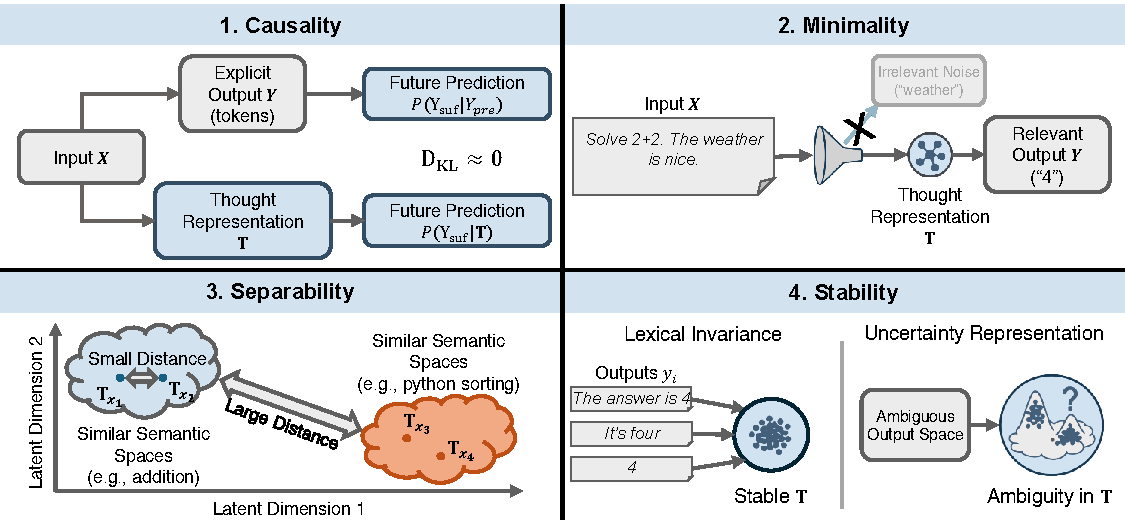
\includegraphics[width=\linewidth]{figures/pdf/characteristics.pdf}
    \vspace{-10pt}
    \caption{Visualizing the axiomatic properties of a Functional Thought Representation $\mathbf{T}$}
    \label{fig:characteristics}
    \vspace{-10pt}
\end{figure}


We identify three gaps that impede principled progress on continuous reasoning. First, there is no \textbf{principled definition} of what a thought representation must do, because existing methods optimize heuristic proxies (step counts, token budgets, imitation of explicit CoT) without a formal statement of the functional requirements. Second, there is no \textbf{intrinsic evaluation} that measures representation quality independently of downstream accuracy~\citep{sahoo2026when}, and therefore failures cannot be attributed to the representation rather than to the decoder or prompt. Third, and consequently, the \textbf{status of current methods} is unknown. Recent audits find that latent reasoning tokens are often unnecessary for the predictions they are meant to drive~\citep{dilgren2026are}, and that latent reasoning does not faithfully implement the structured latent-space search that motivates it~\citep{cui2026how}.

\textbf{Our approach.} We propose an axiomatic characterization of thought representations in terms of four functional properties (\emph{Causality}, \emph{Minimality}, \emph{Separability}, and \emph{Stability}), illustrated in Figure~\ref{fig:characteristics}. The framework describes the function of a thought representation rather than its form. It applies equally to vectors, tensors, or sets of vectors. For each axiom, we define a quantitative measure evaluated directly on the source LLM without retraining. We use this suite to audit candidate thought representations produced by Soft Thinking with and without Gumbel noise~\citep{zhang2025softthinkingunlockingreasoning, wu2026llms} and Latent Thinking~\citep{hao2024training, zou2025latentcollaborationmultiagentsystems} across a range of thinking budgets, alongside candidates extracted from last-input-token hidden states. We study five open-weight LLMs spanning dense and sparse mixture-of-experts architectures on the 23 tasks of Big Bench Extra Hard (BBEH)~\citep{kazemi2025bigbenchextrahard}.

Across the evaluated source LLMs, the intrinsic protocol exposes failure modes that downstream task accuracy does not. The candidates retain coarse task identity but lose the per-question identity that distinguishes one instance of a task from another, and the input-prompt embedding is itself competitive with the candidates on every axis the framework measures.

\textbf{Contributions.} Each of the three gaps above is addressed by a corresponding contribution.
\begin{itemize}
    \item \textbf{Axiomatic formalization of thought representations.} We provide a definition of thought representations stated in terms of four functional axioms, and prove their logical consistency, independence, and completeness (Appendix~\ref{appendix:theoretical_properties}).
    \item \textbf{Intrinsic evaluation protocol.} We introduce a measure for each axiom. KL substitution error measures Causality, the Minimality Gap measures Minimality, same- and cross-task discriminator accuracy measures Separability, and the Distributional Consistency Score (DCS) measures Stability. Each measure is computable on the source LLM without retraining and is decoupled from downstream task accuracy.
    \item \textbf{Empirical audit of candidate thought representations.} Applying the protocol on BBEH exposes a fine-grained \emph{representational collapse} on per-question identity. No evaluated candidate satisfies all four axioms simultaneously, consistent with concurrent reports of silent representational failures in latent reasoning despite unchanged downstream accuracy~\citep{sahoo2026when}.
\end{itemize}

The framework provides a principled means to develop and audit candidate thought representations as objects of study, evaluated for what an LLM encodes about a problem rather than for the downstream reasoning quality of any chain that follows. Beyond evaluation, the four measures provide researchers explicit, quantifiable optimization targets and the diagnostic resolution to attribute downstream accuracy changes to specific representational properties rather than to an aggregate benchmark score. The four measures are one realization of the axioms, which admit alternative quantifications under the same principle, allowing new candidates and measurement designs in future work.
